\PageHeading{07}{四渠道内容与视觉成品}{同一个产品，改变叙事逻辑、图片组织和行动引导}
\begingroup\small
\begin{tabularx}{\linewidth}{P{23mm}Y P{36mm}}
\rowcolor{Forest}\color{white}\bfseries 渠道 & \color{white}\bfseries 内容策略与图文组织 & \color{white}\bfseries 实际交付形态\\
公众号 & 需求背景、事实解释、场景分析与选购建议；2--4张同型号图。 & 内联样式HTML、1200$\times$900封面及ZIP。\\
\rowcolor{Mist}小红书 & 口语标题、短段落、场景清单与话题；3--6张不同原图。 & 3--6页1080$\times$1440 PNG，封面/内容/总结。\\
门店朋友圈 & 一个核心看点与咨询/到店理由；1--3张同型号原图。 & 1080$\times$1080或1080$\times$1440 PNG，独立文案。\\
\rowcolor{Mist}门店海报 & 主副标题、至多3个卖点、核对说明与到店引导；1张主视觉。 & 1080$\times$1920 PNG及来源ZIP。\\
\bottomrule
\end{tabularx}
\endgroup
\vspace{4mm}
\begin{center}
\begin{minipage}[t]{.30\linewidth}\centering
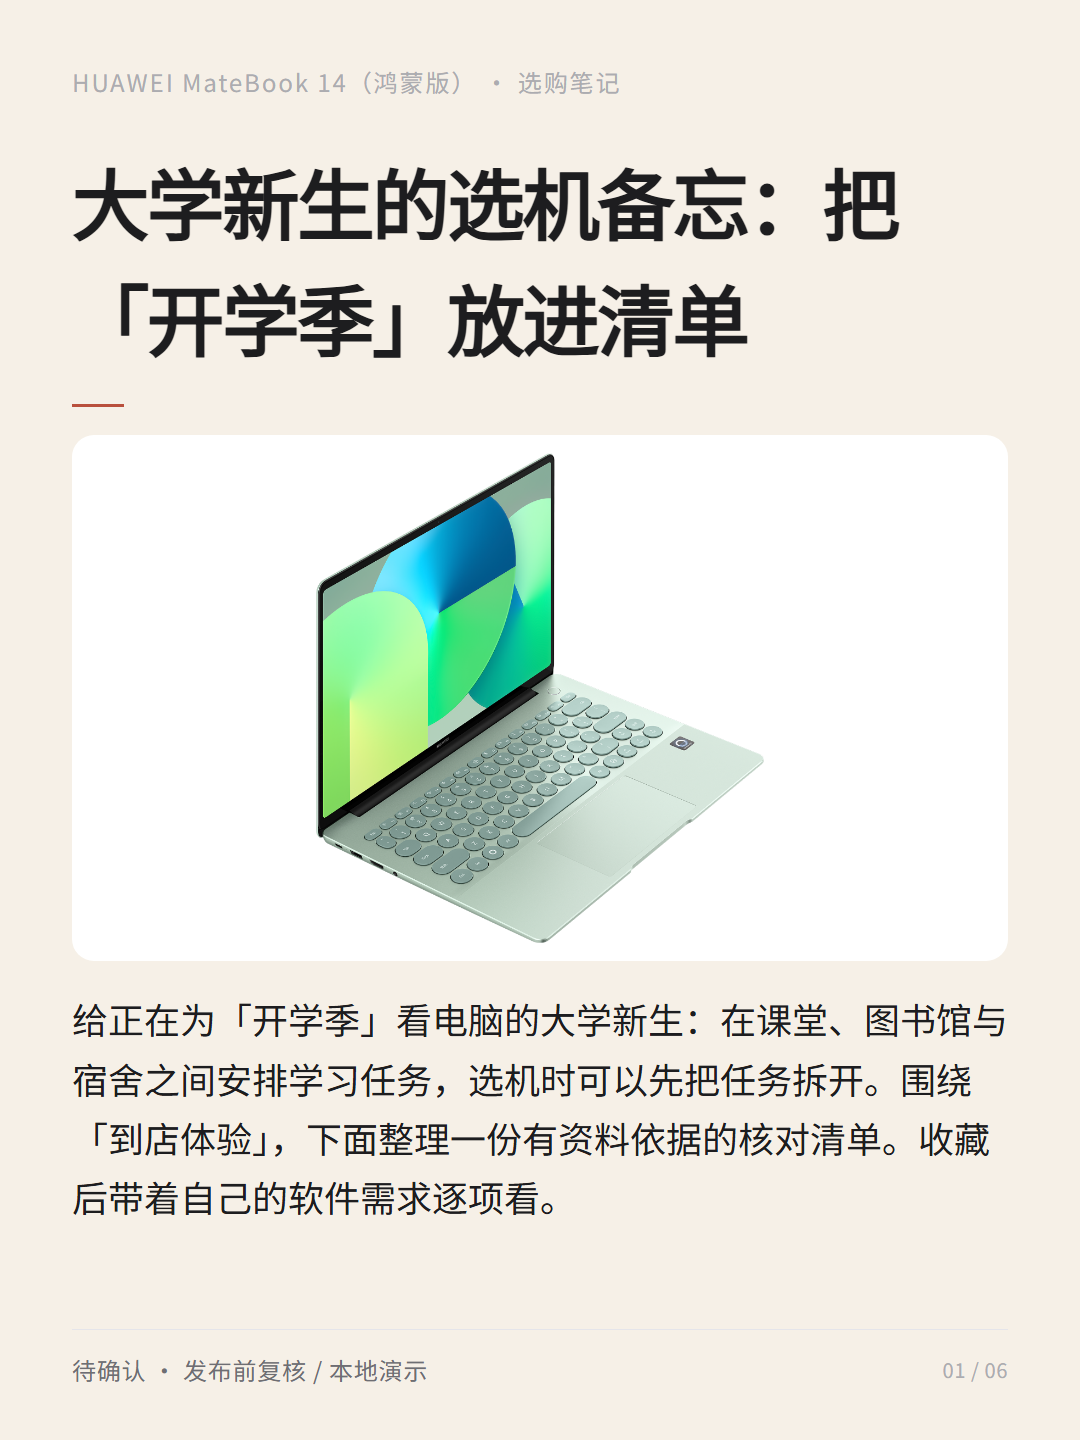
\includegraphics[height=69mm,width=\linewidth,keepaspectratio]{case-a-1.png}\par\small\sffamily 小红书 · 内容封面
\end{minipage}\hfill
\begin{minipage}[t]{.30\linewidth}\centering
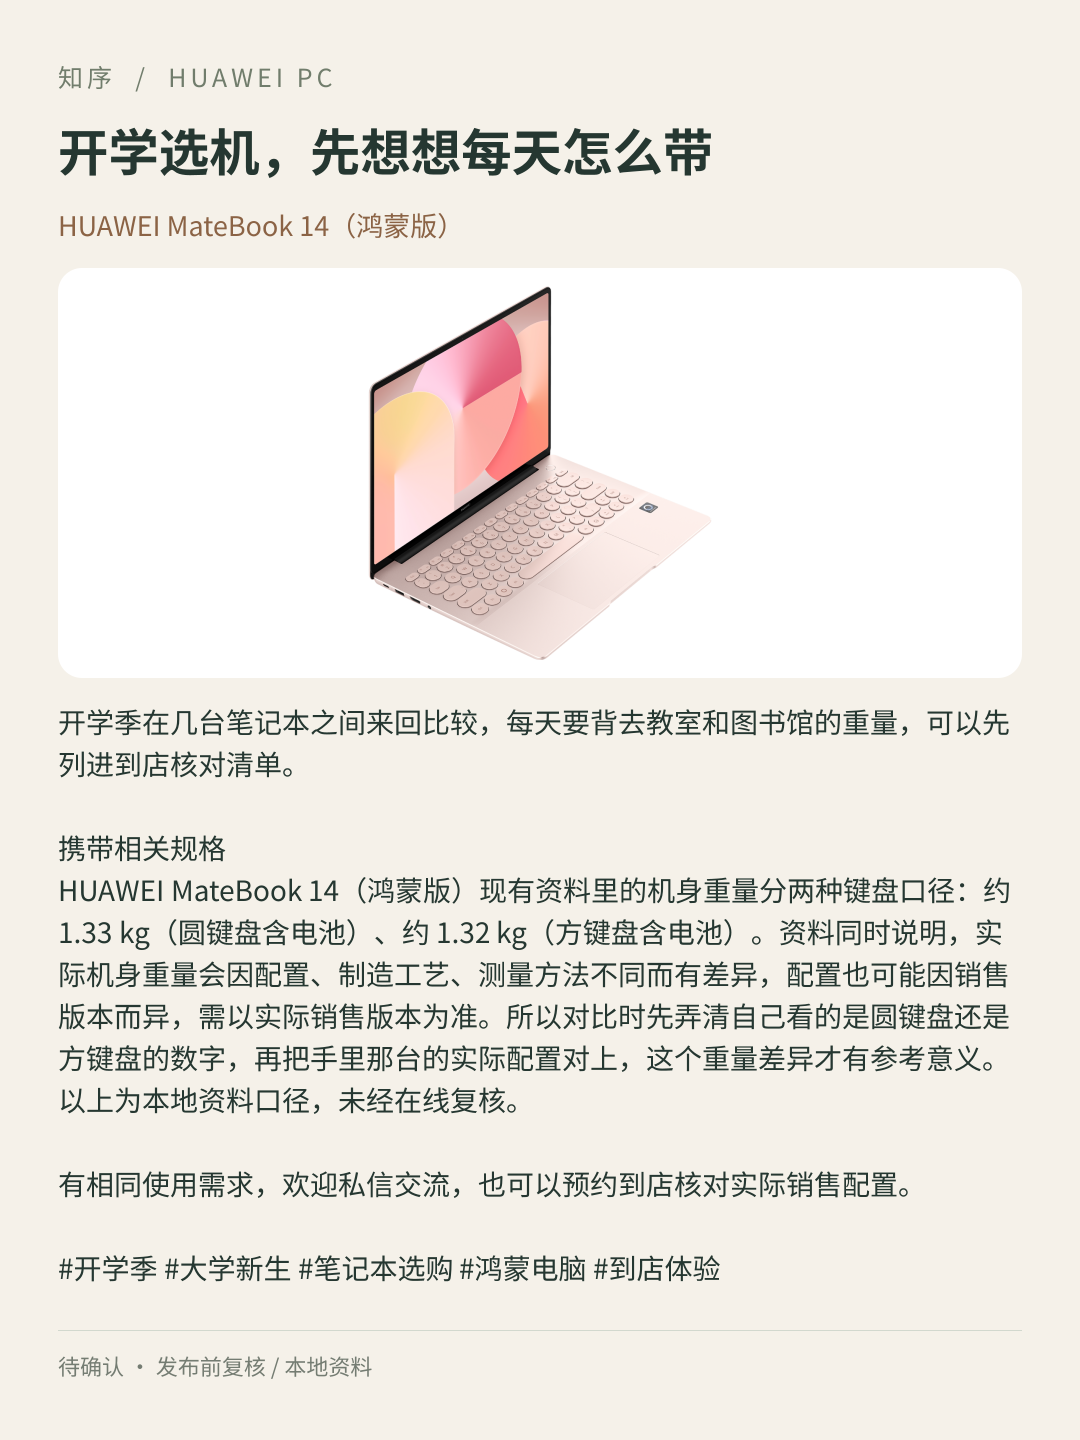
\includegraphics[height=69mm,width=\linewidth,keepaspectratio]{case-c-1.png}\par\small\sffamily 朋友圈 · 场景卡
\end{minipage}\hfill
\begin{minipage}[t]{.30\linewidth}\centering
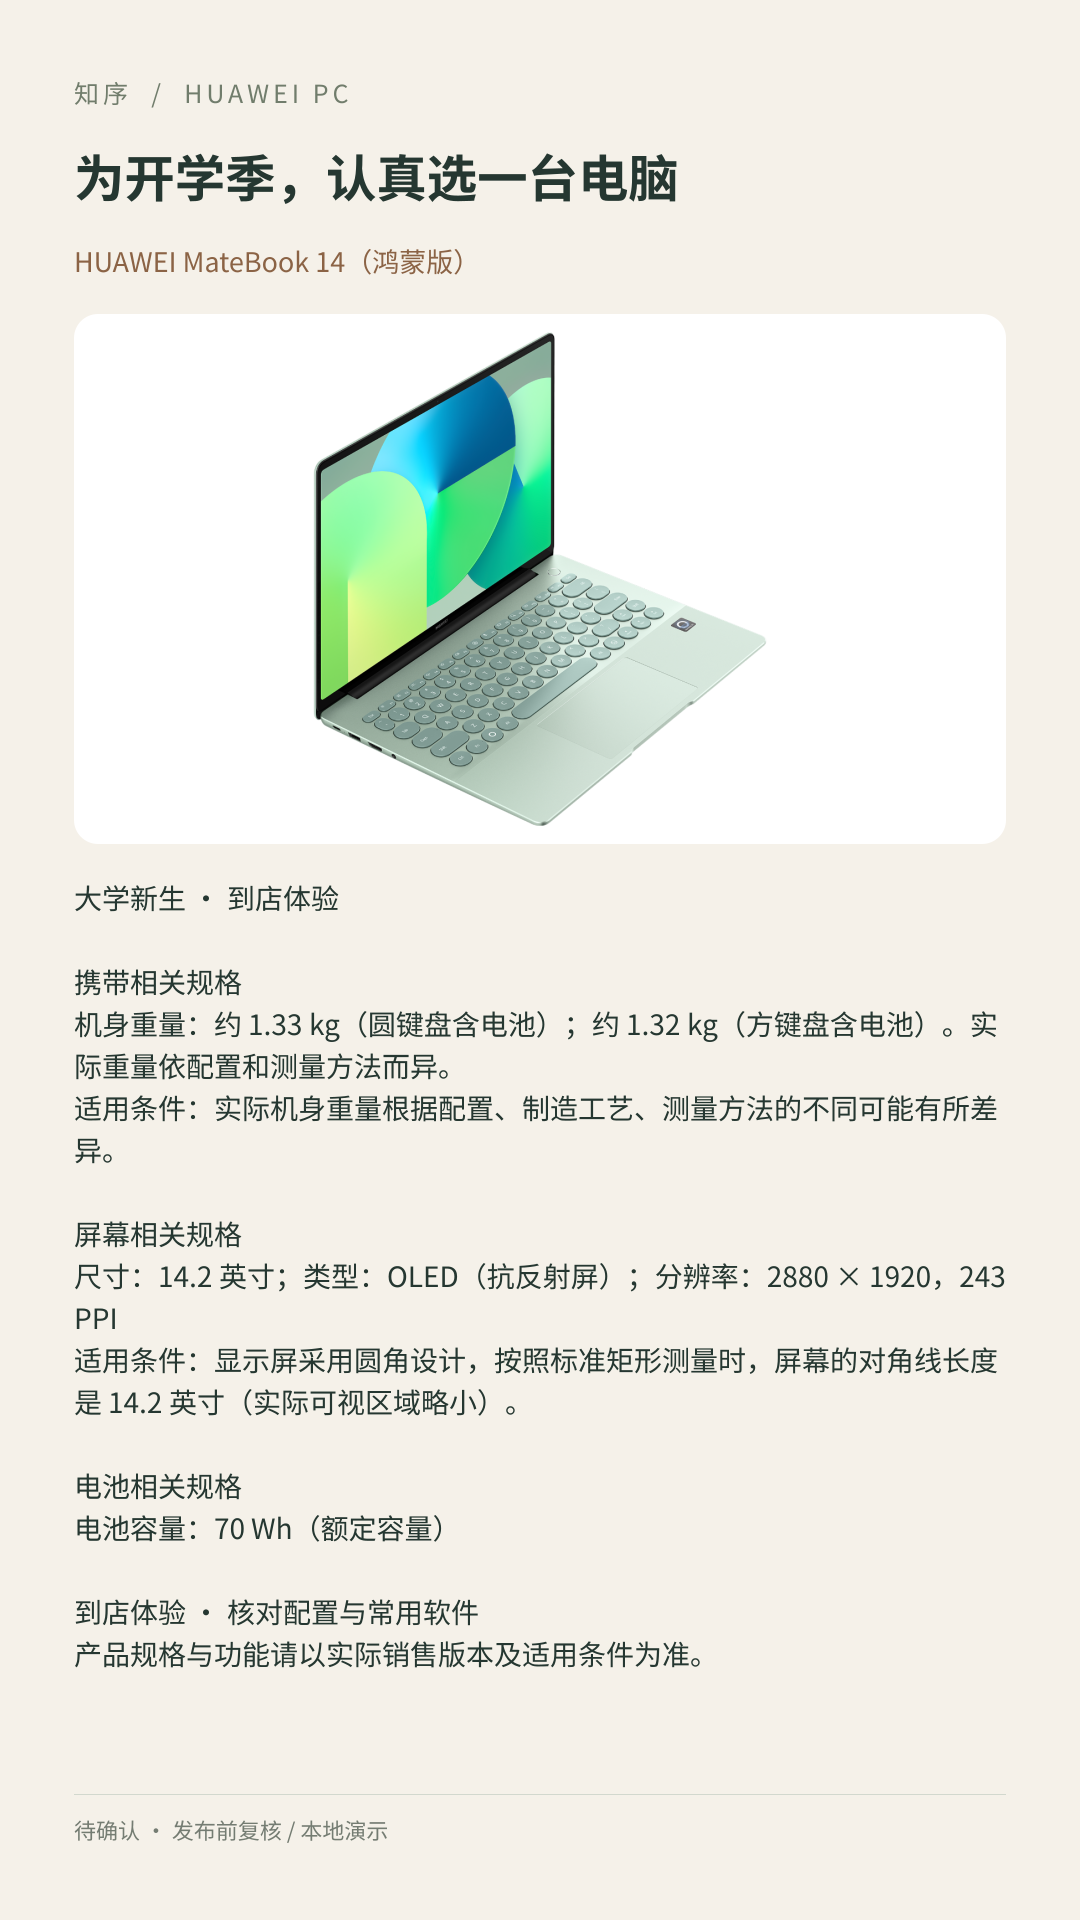
\includegraphics[height=69mm,width=\linewidth,keepaspectratio]{poster.png}\par\small\sffamily 海报 · 主视觉
\end{minipage}
\end{center}
\ImgCap{已生成文件的缩略展示。A与海报为本地规则，C为真实模型+本地资料；均保留待确认/本地来源标记。}
\Sub{渲染与导出的质量约束}
\begin{itemize}
\item 图片从当前证据包解析，保持比例；不拉伸、不重绘设备，不用重复图片凑足数量。
\item 文字按原文排版，保留条件；缩放后仍溢出返回422。选择模板不改变事实审核结论。
\item 公众号以文颜public core排版；小红书采用受控卡片与Chromium；朋友圈/海报由Satori和Sharp生成。
\item ZIP附文案及可读来源/审核说明，省略密钥、临时链接、服务器路径及不透明内部ID。
\end{itemize}
\begin{attention}\small
公众号图片尚未上传微信素材库；粘贴后需上传或替换并复核。当前未完成真实微信编辑器粘贴验收，没有自动发布、印刷PDF或在线图层编辑功能。
\end{attention}
\SourceNote{手册第4页；render模块、第三方许可声明与实际成品核验。模板尺寸是本项目实现选择，不是赛事强制尺寸。}
